
\chapter{Dinic's Algorithm} \label{chap:dnc}

L'algoritmo riprende l'\href{https://en.wikipedia.org/wiki/Edmonds%E2%80%93Karp_algorithm}{Edmonds-Karp} ma invece di incrementare il flusso solo su uno shortest path $P_s$, incrementa il flusso su tutti i path $P_i :\ |P_i| = |P_s|$.
Per semplificare il processo il flusso non viene calcolato sul grafo originale ma bensì sull'\nameref{AdmissibleGraph}

Quindi invece di eseguire una BFS saturare la capacità residua di un solo shortest path e eseguire di nuovo una BFS finche non posso più raggiungere il nodo $t$ da $s$, vengono saturati tutti i path di lunghezza minima ogni volta che si esegue una BFS. Tra una BFS e l'altra viene dunque calcolato un flow che si dice bloccante.
\begin{definition}[Blocking flow]
    Per \textbf{blocking flow} si intende un flusso su un grafo (in questo caso il residuo del level graph) che satura almeno un arco per ogni possibile \textit{path} da $s\rightarrow t$.    
\end{definition}
L'algoritmo prende in input il network e la funzione che attribuisce ad ogni arco una capacità.
Viene creata una funzione che associa ad ogni arco il flow che lo attraversa.
Per leggibilità a brevità il grafo residuo e segnato come $G_f$ che indica il grafo residuo in cui è instradato il flow $f$ aggiornato al momento in cui vi si fa riferimento.
La BFS prende in input il grafo residuo e dunque non considera archi saturati.
\begin{algorithm}
    \caption{\textit{Dinics-Algorithm(G, c)}}
    \label{algotrans}
    \begin{algorithmic}[1]
        \State $f_{ij} = 0 \forall (i,j)\in E(G)$ 
        \State $d =  BFS(G_f)$
        
        \While{$d(s) \not = \infty$}
            \State $\delta = \min_{\forall (i,j)\in P} c(i,j)$
            \State $f_{ij} = f_{ij}+\delta\ \forall (i,j)\in P$
            \State $P = findPathSoLong(G_f,d(s))$
            \If{$P = \varnothing$} 
                \State $d =  BFS(G_f)$
            \EndIf
        \EndWhile 
        \State return $f$
    \end{algorithmic}
\end{algorithm}


Sia $x = dist_i(s,t)$ la distanza da $s$ a $t$ in una certa iterazione $i$ del dinic's algorithm e siano $P_0, ..., P_k$ tutti i $k$ percorsi $s\rightarrow t$ di lunghezza $x$ allora in ogni
 ma ragionando sul fatto che ogni volta che eseguo una BFS creo un albero di copertura con \underline{livelli} che indicano la distanza dal nodo di partenza.
quindi invece di eseguire una BFS e poi saturare solo uno dei percorsi minimi trovati, posso saturarli tutti prima di eseguire di nuovo una BFS.
Ogni volta che si esegue una BFS dalla \textit{source} si entra nella \textbf{blocking flow phase}.\\

\begin{obs}{Max flow $\implies$ blocking flow}{}
    Il max flow è un blocking flow ma non è vera l'implicazione opposta.
\end{obs}
per \textbf{level graph} si intende l'albero di copertura dato da una BFS che riporta per ogni nodo la distanza dalla radice, dividendo così il grafo in livelli.
\begin{center}
    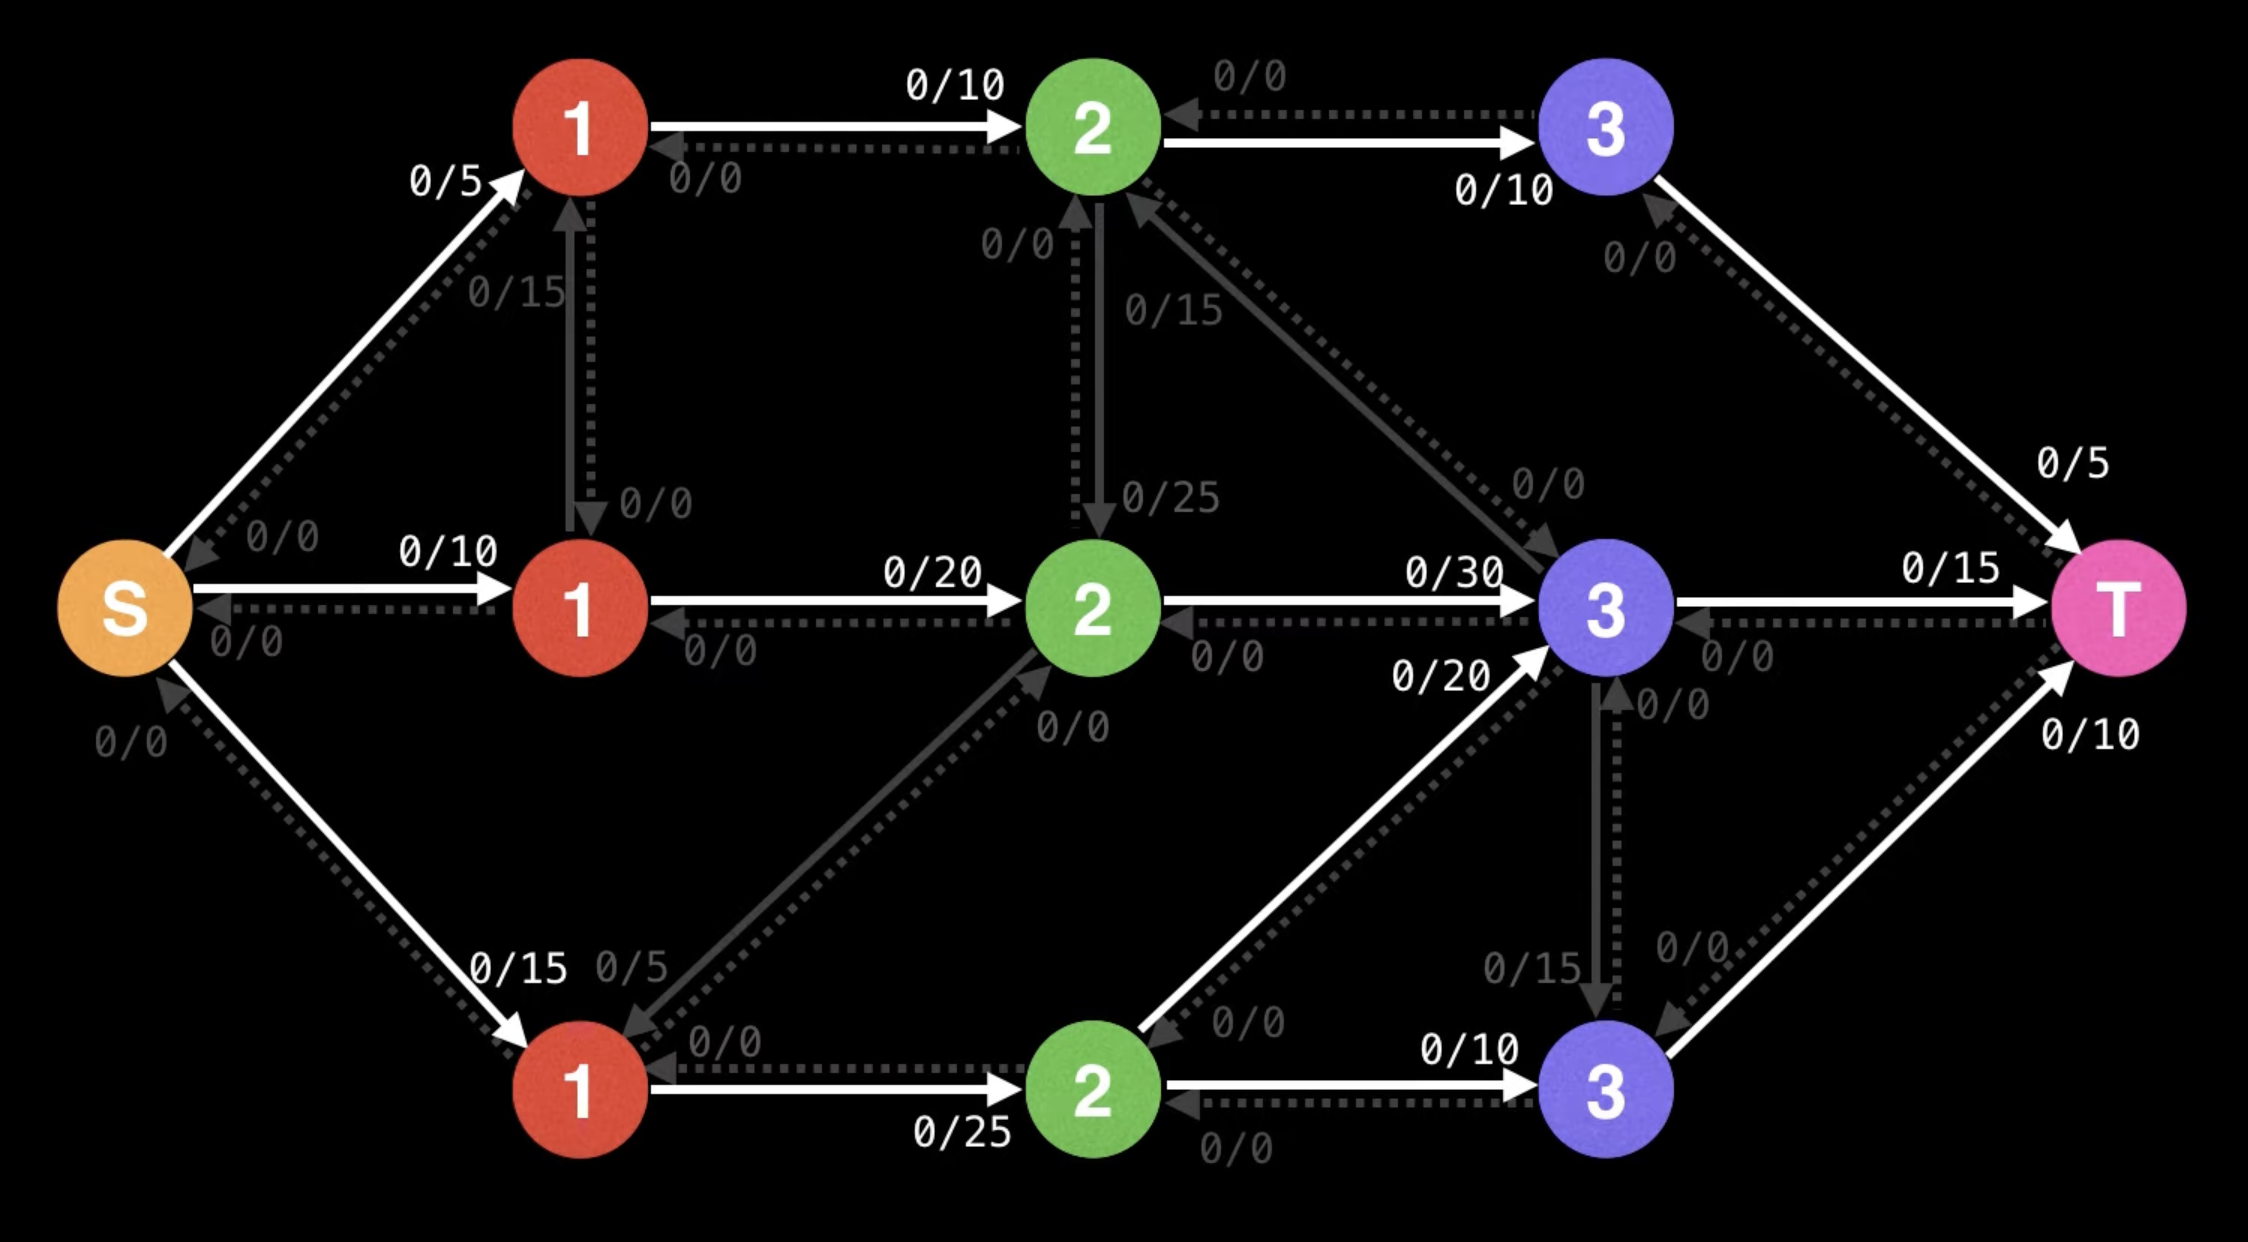
\includegraphics[height=5.25cm]{resources/images/levelGraph.png}\\
    \textit{source: \href{https://www.youtube.com/watch?v=M6cm8UeeziI&t=2s}{Dinic's Algorithm by WilliamFriset}}
\end{center}
In questo modo si riduce il costo dell'algoritmo da $O(n^2m)$ per Edmonds Karp a $O(nm^2)$
\paragraph{Altri link utili}\begin{enumerate}
    \item \href{http://courses.csail.mit.edu/6.854/16/Notes/n10-blocking_flows.html}{Lecture from MIT}
    \item \href{https://en.wikipedia.org/wiki/Dinic%27s_algorithm}{Wikipedia}
\end{enumerate}

\cleardoublepage

